%!TEX root = ../thesis.tex

% \section{背景}
% \subsection{RoboCup}
マニピュレータには正しい図の描き方がある.図に描いたマニピュレータの例を以下の
図 1 に示す.(a)と(b)はそれぞれ 2 自由度のマニピュレータを表しており,角度$\theta$と
長さ$\l$の矢印以外は同じである.角度$\theta$についてはプラスとマイナスがあるため,矢印の
方向に気を付ける必要がある.よって,(b)のような矢印の描き方が望まれる.また,長
さ$\l$についてはプラスしかないため,これも(b)のような矢印の描き方が望まれる.
\begin{figure}[hbtp]
  \centering
 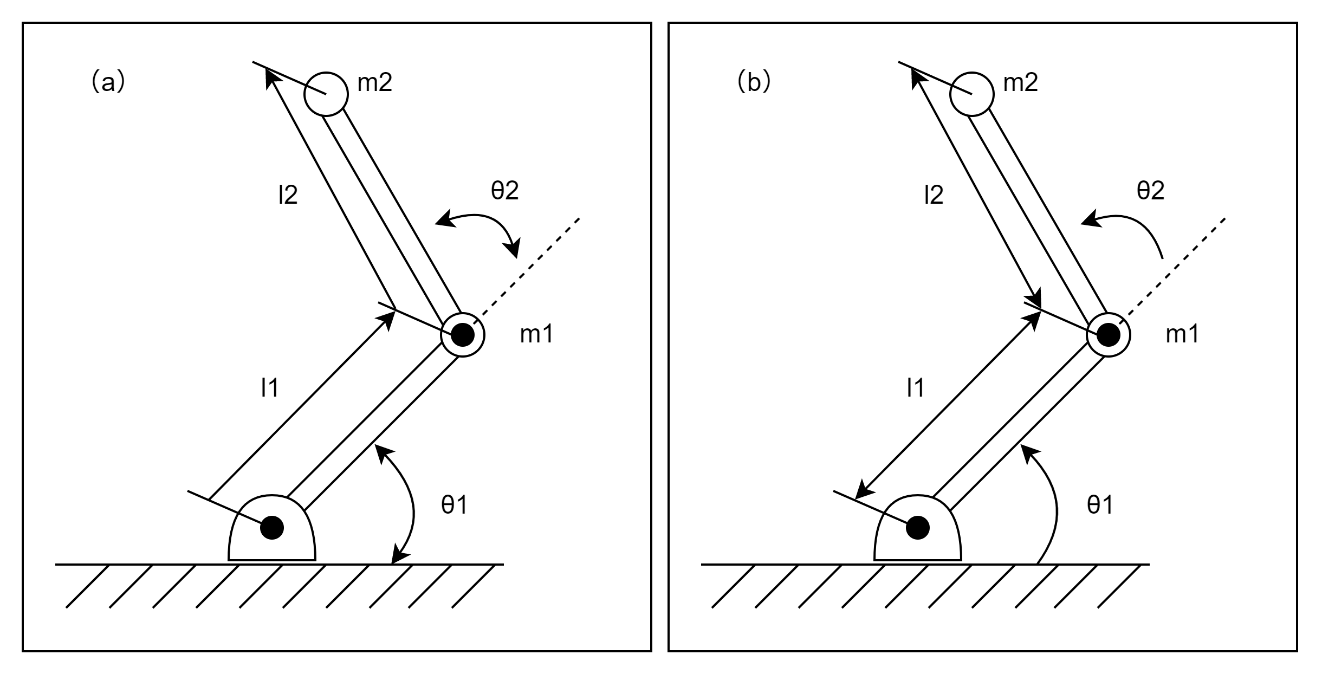
\includegraphics[keepaspectratio, scale=0.8]
      {images/mani.png}
 \caption{Manipulator}
 \label{Fig:manipulator}
\end{figure}

\newpage
